% article example for classicthesis.sty
\documentclass[11pt,a4paper]{scrartcl} % KOMA-Script article 
\usepackage{lipsum}
\usepackage{url}
\usepackage[LabelsAligned]{currvita} % nice cv style
\usepackage[nochapters]{classicthesis} % nochapters
\usepackage{tikz}
\usepackage{amsthm}
\usepackage{setspace}
\usepackage{pifont}
\usepackage{color}
\usepackage{graphicx}
\usepackage{natbib}
\usetikzlibrary{calc,shapes,arrows,automata,trees,shadows,decorations.pathmorphing,positioning,
shapes.misc,shapes.arrows,chains,matrix,scopes,decorations.pathmorphing,backgrounds}
\renewcommand*{\cvheadingfont}{\LARGE\color{Maroon}}
\renewcommand*{\cvlistheadingfont}{\large}
\renewcommand*{\cvlabelfont}{\qquad}
\DeclareGraphicsExtensions{.pdf,.png,.jpg}
\begin{document}
\pagecolor{Sepia!20}
%Coverletter
\begin{cv}{\spacedallcaps{Unseen}}
        \begin{cvlist}{\textcolor{brown}{\spacedlowsmallcaps{Jason~N~Mansfield}}}\label{PersDat}  
            \item   Regis University
            \item   3333\\
                    Regis Boulevard Denver \\	
                    Colorado 80221-1099
            \item   mansf843@regis.edu\\				
                    \url{http://www.regis.edu/}				
        \end{cvlist}
        \begin{cvlist}{\spacedlowsmallcaps{RC~471}}\label{irgendwas}
            \item Instructed by Professor~Henri~Tshibambe\\
             \url{http://tinyurl.com/3htorkr}
        \end{cvlist}
    \end{cv}
\clearpage
\noindent
\begin{center}
\textcolor{Maroon}{\spacedallcaps{NIV Archaeological Study Bible~\cite{niv}}}\\
\textcolor{Maroon}{\spacedlowsmallcaps{PSALMS~143}}\\
\begin{verse}
5 I remember† the days of long ago; I meditate on all your works and consider what your hands have done. \\
6 I spread out my hands† to you; my soul thirsts for you like a parched land.\\ 
Selah 
\end{verse}
\end{center}

\clearpage
%Title
\title{\textcolor{Maroon}{\rmfamily\normalfont\spacedallcaps{Unseen}}}
    \author{\textcolor{brown}{\spacedlowsmallcaps{Jason N Mansfield}}}
    \date{} % no date
    
    \maketitle
    
 \begin{abstract}
Throughout our busy daily lives we form assumptions of what is important. Most have forgotten the most important practice during their busy day. Without removing ourselves from all our distractions, blast of media combined with advertising and stress from money and job issues there is never time for prayer or meditation. There are a few techniques which if practiced properly can strengthen our ability to understand ourself and the creator who lovingly created us. These practices can help reveal both the unseen in our creator and within ourselves.
 \end{abstract}
       
    \tableofcontents

\section{Spirit}
\begin{center}
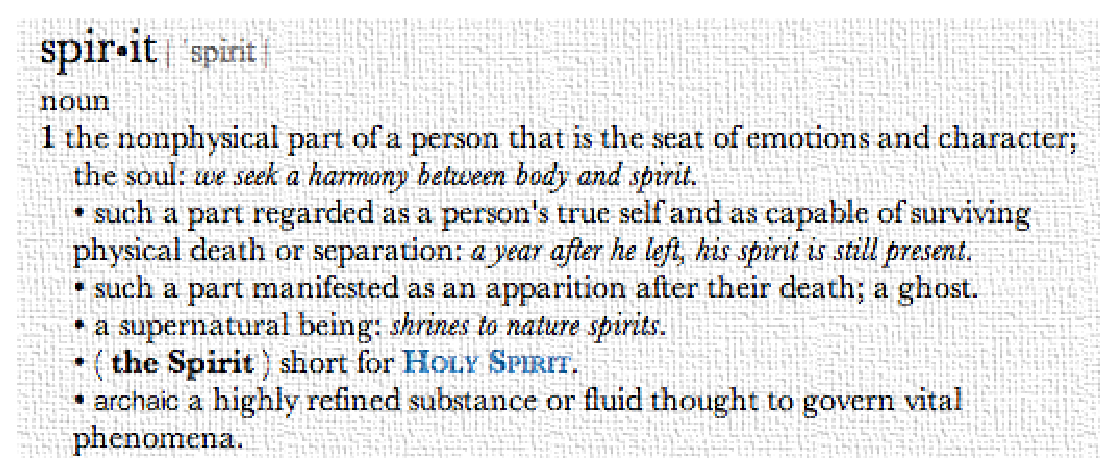
\includegraphics[scale=0.5]{spirit}\\
\end{center}
\begin{doublespace}
The spirit~\cite{wiki:000} is an English word derived from Latin spiritus~\cite{wiki:001} or breath. Within this spirit lies a path to its immaterial meaning or sacred purpose. In order to walk this path we require guidance and spiritual tools. For Christian based faith we have God's word in the Bible but it takes more than this gift. God has also given us his word in the world around us. God's word is written in the Mountains and their majestic terrain. God's word is written in the teaming species moving through the Oceans. God's word in in your child's eyes and laughter. God is in your heart. In our daily life its easy to forget we are crafted in God's image:
\end{doublespace}  
\begin{verse}
\textcolor{Maroon}{\spacedlowsmallcaps{GENESIS~1}}\\
26 Then God said, “Let us† make man in our image,† in our likeness, and let them rule† over the fish of the sea and the birds of the air, over the livestock, over all the earth, and over all the creatures that move along the ground.” 
\end{verse}
\begin{doublespace}
How can we then tap into the resources God has given us to develop an understanding of ourselves? Many believe Meditation is a useful tool which opens up this connection between the individual and God. Meditation? You might question. Isn't this a practice used by Eastern Religions such as Buddhists? The distinction lies in the opposite approaches used. Buddhists us meditation to empty the mind. Christians use meditation to fill their minds~\cite{wiki:003}. 
\section{Silence and Solitude}
Christian can also learn the importance of silence during this practice. Edmund P. Clowney~\cite{clowney2002christian} had this to say regarding our father in heaven:
\end{doublespace}
\begin{quotation}
Christian meditation has always stood silent by the cross, hearing the cry of the Son: "My God, my God, why hast thou forsaken me?" (Mark 15:34); but hearing also the silence of the Father as he forsook his only begotten Son, the only Man who did not deserve to be forsaken. Again, we can only meditate on the price that the Father paid in the darkness of Golgotha.
\end{quotation}
\begin{doublespace}
This is a pretty powerful statement which emphasis how meaningful silence can really be. If God himself was silent during the horror of this event; how important is it for our silence and contemplation during our thoughts about spiritual matters? Hesychasm~\cite{wiki:004} which is Greek for silence or rest is an eremitic tradition of prayer. This style of prayer is shown in guidance from Jesus within the Gospel of Matthew:
\end{doublespace}
\begin{verse}
\textcolor{Maroon}{\spacedlowsmallcaps{MATTHEW~6}}\\
5 “And when you pray, do not be like the hypocrites, for they love to pray standing† in the synagogues and on the street corners to be seen by men. I tell you the truth, they have received their reward in full.\\
6 But when you pray, go into your room, close the door and pray to your Father,† who is unseen. Then your Father, who sees what is done in secret, will reward you. 
\end{verse}
\begin{doublespace}
This instruction seems to encourage a form of solitude as well as silence. This is not because we want to be silent about Gods word but silent when seeking him on a personal level and for pure reasons. This solitude allows us to block out the outside world and concentrate on our purpose in the scheme of life.  Solitude from people and other distractions allows the individual in prayer to truly seek the holy spirit. 
\section{Imagination}
An excellent example of human imagination being used in prayer was the formation of Spiritual Exercises discovered by a wounded Spanish knight who became a Saint~\cite{wiki:005} . Saint Ignatius of Loyola's Spiritual Exercises are broken into Four weeks of soul searching and prayer. This discipline encourages the use of imagination to fully grasp the magnitude of choices made within an individuals life. The following is taken from The Spiritual Exercises of St. Ignatius of Loyola in Kindle Locations 935-944~\cite{Ignatius}:
\end{doublespace}
\textcolor{Maroon}{\spacedlowsmallcaps{The~Fifth~Exercise}}\\
\begin{verse}
The preparatory prayer does not differ from that above. The first prelude is here the forming of the place; which is to set before the eyes of the imagination the length, breadth, and depth of hell.\\
\end{verse}
\begin{verse}
The second consists in asking for an intimate perception of the punishments which the damned undergo ; that, if at any time I should be forgetful of the love of God, at least the fear of punishment may restrain me from sins.
\end{verse}
\begin{verse}
The first point is, to see by the imagination the vast fires of hell, and the souls enclosed in certain fiery bodies, as it were in dungeons.*
\end{verse}
\begin{verse}
The second, to hear in imagination the lamentations, the howlings, the exclamations, and the blasphemies against Christ and His saints, thence breaking forth.
\end{verse}
\begin{verse}
The third, to perceive by the smell also of the imagination, the smoke, the brim stone, and the stench of a kind of sink or filth, and of putrefaction. 
\end{verse}
\begin{doublespace}
While an unpleasant picture is brought to mind in this fifth exercise other exercises are concerning more encouraging imaginative meditations. All of Saint Ignatius's exercises are meant to strengthen the individual through disciplined topics in organized form. Stemming from this use of imagination one may use imagination to visualize a variety of topics which can motivate them spiritually such as Christs caring for the poor or Sermon on the Mount.
\end{doublespace}
\section{Nature}
\begin{verse}
\textcolor{Maroon}{\spacedlowsmallcaps{GENESIS~1}}\\
20 And God said, “Let the water teem with living creatures, and let birds fly above the earth across the expanse of the sky.” \\
21 So God created the great creatures of the sea and every living and moving thing with which the water teems,† according to their kinds, and every winged bird according to its kind. And God saw that it was good. \\
22 God blessed them and said, “Be fruitful and increase in number and fill the water in the seas, and let the birds increase on the earth.”† 
\end{verse}
\begin{doublespace}
God is unseen but shown through his creations in many ways. God reveals himself through his creations and the complexity of this world around us. That does not mean we should lock ourselves in a physical box and claim we are limited to it. Author Gerald Schroeder~\cite{GLSchroeder-2001} neatly describes the common confusion people confront in modern society where spirituality has been drained of its purpose or true understanding:
\end{doublespace}
\begin{quote}
Logic alone tells you it could not have happened by chance. But the materialist superstition of our culture, the idea that if you can’t measure it, it’s not there, insists that chance be the explanation. And once a fact is imprinted on a mind, like the song a sparrow learns in its youth, that fact is yours for life. Believe it or not! And yet here we are. A small part of a vast universe thinking about its origins, rummaging through steamer trunks in the attics of space and brain, trying to find the meaning of that which we call the mind. 
\end{quote}
\begin{doublespace}
Nature was never intended to be treated as it has been by man. The few that explore and take care of it properly begin to tap into the connection originally meant for man. This is another form of understanding helps you understand yourself better and God's original task for you as an individual. Men were to be gardeners of earth not its destroyers. Spending time in touch with Nature is an excellent way to also approach God by appreciating his intelligent designs which have branched out into millions of various forms since inception. The natural world is also an excellent place to practice all of these techniques and may sometimes be the only place you can find solitude or silence. 
\section{Practice}
Combining Silence, Solitude and Nature is no automatic connection to the Holy Spirit but making use of these techniques is a start. For generations man has tried to put down in writing a variety of techniques but its these techniques with a valid effort to know and serve God that matters. Moses set a good example for us as shown in the powerful connection he had with God in prayer:
\begin{verse}
\textcolor{Maroon}{\spacedlowsmallcaps{EXODUS~9}}\\
29 Moses replied, “When I have gone out of the city, I will spread out my hands† in prayer to the LORD. The thunder will stop and there will be no more hail, so you may know that the earth† is the LORD’s. 
\end{verse} 
\end{doublespace}
\clearpage
  % bib stuff
    \nocite{*}
    \addtocontents{toc}{\protect\vspace{\beforebibskip}}
    \addcontentsline{toc}{section}{\refname}    
    \bibliographystyle{plain}
    \bibliography{cite}
\end{document}